 
\begin{enumerate}
\begin{multicols}{2}
 \item Pavé droit (ou parallélépipède rectangle):\\
$V=largeur \times longueur \times hauteur$
\begin{center}
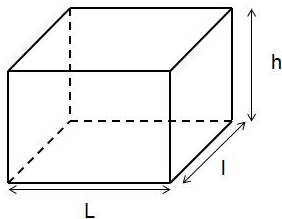
\includegraphics[scale=0.4]{RepS-pave_droit.png} 
\end{center} 


\item Prisme droit:\\  $V=A_{base} \times hauteur$

\begin{center}
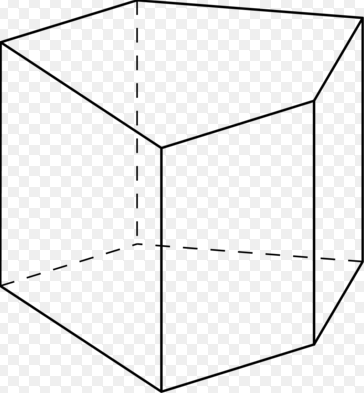
\includegraphics[scale=0.2]{RepS-prisme_droit.png} 
\end{center}


\item  Cylindre:\\ 
$V=A_{base} \times hauteur = \pi R^2 \times hauteur$

\begin{center}
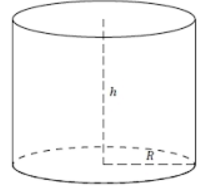
\includegraphics[scale=0.4]{RepS-cylindre.png} 
\end{center}


\item Pyramide:\\ $V= \frac{ A_{base} \times hauteur}{3}$

\begin{center}
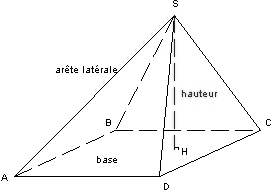
\includegraphics[scale=0.5]{RepS-pyramide.png} 
\end{center}

\item Cône de révolution:\\
$V=\frac{ A_{base} \times hauteur}{3}=\frac{ \pi \times R^2 \times hauteur}{3}$

\begin{center}
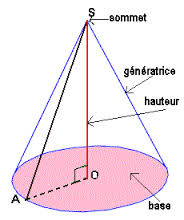
\includegraphics[scale=0.3]{RepS-cone.png} 
\end{center}
\end{multicols}
\end{enumerate}
